%%%%%%%%%%%%%%%%%%%%%%%%%%%%%%%%%%%%%%%%%
% Classicthesis Typographic Thesis
% LaTeX Template
% Version 1.1 (4/8/12)
%
% This template has been downloaded from:
% http://www.LaTeXTemplates.com
%
% Original author:
% André Miede (http://www.miede.de)
%
% License:
% CC BY-NC-SA 3.0 (http://creativecommons.org/licenses/by-nc-sa/3.0/)
%
% General Tips:
% 1) Make sure to edit the classicthesis-config.file
% 2) New enumeration (A., B., C., etc in small caps): %\begin{aenumerate} \end{aenumerate}
% 3) For margin notes: \marginpar or \graffito{}
% 4) Do not use bold fonts in this style, it is designed around them
% 5) Use tables as in the examples
% 6) See classicthesis-preamble.sty for useful commands
%
%%%%%%%%%%%%%%%%%%%%%%%%%%%%%%%%%%%%%%%%%

%----------------------------------------------------------------------
%	PACKAGES AND OTHER DOCUMENT CONFIGURATIONS
%---------------------------------------------------------------------

\documentclass[
		oneside,openright,titlepage,numbers=noenddot,headinclude,%1headlines,
                footinclude=true,cleardoublepage=empty,
                BCOR=5mm,paper=a4,fontsize=12pt, % Binding correction, paper type and font size
                american, % Languages
                ]{scrreprt} 
                
% Includes the file which contains all the document configurations and packages - make sure to edit this file
%%%%%%%%%%%%%%%%%%%%%%%%%%%%%%%%%%%%%%%%%
% Thesis Configuration File
%
% The main lines to change in this file are in the DOCUMENT VARIABLES
% section, the rest of the file is for advanced configuration.
%
%%%%%%%%%%%%%%%%%%%%%%%%%%%%%%%%%%%%%%%%%

%----------------------------------------------------------------------------------------
%	DOCUMENT VARIABLES
%	Fill in the lines below to enter your information into the thesis template
%	Each of the commands can be cited anywhere in the thesis
%----------------------------------------------------------------------------------------

% Remove drafting to get rid of the '[ Date - classicthesis version 4.0 ]' text at the bottom of every page
\PassOptionsToPackage{eulerchapternumbers,subfig,beramono,eulermath,subfig,drafting}{classicthesis}
% Available options: drafting parts nochapters linedheaders eulerchapternumbers beramono eulermath pdfspacing minionprospacing tocaligned dottedtoc manychapters listings floatperchapter subfig
% Adding 'dottedtoc' will make page numbers in the table of contents flushed right with dots leading to them

\newcommand{\myTitle}{A Classic Thesis Style\xspace}
\newcommand{\mySubtitle}{An Homage to The Elements of Typographic Style\xspace}
\newcommand{\myDegree}{Doktor-Ingenieur (Dr.-Ing.)\xspace}
\newcommand{\myName}{Andr\'e Miede\xspace}
\newcommand{\myProf}{Put name here\xspace}
\newcommand{\myOtherProf}{Put name here\xspace}
\newcommand{\mySupervisor}{Put name here\xspace}
\newcommand{\myFaculty}{Put data here\xspace}
\newcommand{\myDepartment}{Put data here\xspace}
\newcommand{\myUni}{Put data here\xspace}
\newcommand{\myLocation}{Darmstadt\xspace}
\newcommand{\myTime}{December 2011\xspace}
\newcommand{\myVersion}{version 4.0\xspace}

%----------------------------------------------------------------------------------------
%	USEFUL COMMANDS
%----------------------------------------------------------------------------------------

\newcommand{\ie}{i.\,e.}
\newcommand{\Ie}{I.\,e.}
\newcommand{\eg}{e.\,g.}
\newcommand{\Eg}{E.\,g.} 

\newcounter{dummy} % Necessary for correct hyperlinks (to index, bib, etc.)
\providecommand{\mLyX}{L\kern-.1667em\lower.25em\hbox{Y}\kern-.125emX\@}

%----------------------------------------------------------------------------------------
%	PACKAGES
%----------------------------------------------------------------------------------------
% Added by Lisa

% font select changes
\usepackage{everysel}
% linguistic examples
% http://en.wikibooks.org/wiki/LaTeX/Linguistics#Enumerated_examples
\usepackage{linguex}
%\usepackage{gb4e}
%----------------------------------------------------------------------------------------

\usepackage{lipsum} % Used for inserting dummy 'Lorem ipsum' text into the template

%------------------------------------------------
 
\PassOptionsToPackage{latin9}{inputenc} % latin9 (ISO-8859-9) = latin1+"Euro sign"
\usepackage{inputenc}
 
 %------------------------------------------------

%\PassOptionsToPackage{ngerman,american}{babel}  % Change this to your language(s)
% Spanish languages need extra options in order to work with this template
%\PassOptionsToPackage{spanish,es-lcroman}{babel}
\usepackage{babel}

%------------------------------------------------			


%\usepackage[nosectionbib]{apacite}

\usepackage{apacite}
\usepackage{makerobust}
\DeclareRobustCommand{\citep}[2][]{\cite[#1]{#2}}
\DeclareRobustCommand{\citealp}[2][]{\citeNP[#1]{#2}}
\DeclareRobustCommand{\citet}[2][]{\citeA[#1]{#2}}
\MakeRobustCommand{\citeauthor}
\MakeRobustCommand{\citeauthor}

\PassOptionsToPackage{round}{natbib}
\usepackage{natbib}

 %------------------------------------------------

\PassOptionsToPackage{fleqn}{amsmath} % Math environments and more by the AMS 
 \usepackage{amsmath}
 
 %------------------------------------------------

\PassOptionsToPackage{T1}{fontenc} % T2A for cyrillics
\usepackage{fontenc}

%------------------------------------------------

\usepackage{xspace} % To get the spacing after macros right

%------------------------------------------------

\usepackage{mparhack} % To get marginpar right

%------------------------------------------------

\usepackage{fixltx2e} % Fixes some LaTeX stuff 

%------------------------------------------------

\PassOptionsToPackage{smaller}{acronym} % Include printonlyused in the first bracket to only show acronyms used in the text
\usepackage{acronym} % nice macros for handling all acronyms in the thesis

%------------------------------------------------

%\renewcommand*{\acsfont}[1]{\textssc{#1}} % For MinionPro
\renewcommand{\bflabel}[1]{{#1}\hfill} % Fix the list of acronyms

%------------------------------------------------

\PassOptionsToPackage{pdftex}{graphicx}
\usepackage{graphicx} 

%----------------------------------------------------------------------------------------
%	FLOATS: TABLES, FIGURES AND CAPTIONS SETUP
%----------------------------------------------------------------------------------------

\usepackage{tabularx} % Better tables
\setlength{\extrarowheight}{3pt} % Increase table row height
\newcommand{\tableheadline}[1]{\multicolumn{1}{c}{\spacedlowsmallcaps{#1}}}
\newcommand{\myfloatalign}{\centering} % To be used with each float for alignment
\usepackage{caption}
\captionsetup{format=hang,font=small}
\usepackage{subfig}  

%----------------------------------------------------------------------------------------
%	CODE LISTINGS SETUP
%----------------------------------------------------------------------------------------

\usepackage{listings} 
%\lstset{emph={trueIndex,root},emphstyle=\color{BlueViolet}}%\underbar} % for special keywords
\lstset{language=[LaTeX]Tex, % Specify the language for listings here
keywordstyle=\color{RoyalBlue}, % Add \bfseries for bold
basicstyle=\small\ttfamily, % Makes listings a smaller font size and a different font
%identifierstyle=\color{NavyBlue}, % Color of text inside brackets
commentstyle=\color{Green}\ttfamily, % Color of comments
stringstyle=\rmfamily, % Font type to use for strings
numbers=left, % Change left to none to remove line numbers
numberstyle=\scriptsize, % Font size of the line numbers
stepnumber=5, % Increment of line numbers
numbersep=8pt, % Distance of line numbers from code listing
showstringspaces=false, % Sets whether spaces in strings should appear underlined
breaklines=true, % Force the code to stay in the confines of the listing box
%frameround=ftff, % Uncomment for rounded frame
frame=single, % Frame border - none/leftline/topline/bottomline/lines/single/shadowbox/L
belowcaptionskip=.75\baselineskip % Space after the "Listing #: Desciption" text and the listing box
}

%----------------------------------------------------------------------------------------
%	HYPERREFERENCES
%----------------------------------------------------------------------------------------

\PassOptionsToPackage{pdftex,hyperfootnotes=false,pdfpagelabels}{hyperref}
\usepackage{hyperref}  % backref linktocpage pagebackref
\pdfcompresslevel=9
\pdfadjustspacing=1

\hypersetup{
% Uncomment the line below to remove all links (to references, figures, tables, etc)
%draft, 
colorlinks=true, linktocpage=true, pdfstartpage=3, pdfstartview=FitV,
% Uncomment the line below if you want to have black links (e.g. for printing black and white)
%colorlinks=false, linktocpage=false, pdfborder={0 0 0}, pdfstartpage=3, pdfstartview=FitV, 
breaklinks=true, pdfpagemode=UseNone, pageanchor=true, pdfpagemode=UseOutlines,
plainpages=false, bookmarksnumbered, bookmarksopen=true, bookmarksopenlevel=1,
hypertexnames=true, pdfhighlight=/O, urlcolor=webbrown, linkcolor=RoyalBlue, citecolor=webgreen,
%------------------------------------------------
% PDF file meta-information
pdftitle={\myTitle},
pdfauthor={\textcopyright\ \myName, \myUni, \myFaculty},
pdfsubject={},
pdfkeywords={},
pdfcreator={pdfLaTeX},
pdfproducer={LaTeX with hyperref and classicthesis}
%------------------------------------------------
}   

%----------------------------------------------------------------------------------------
%	BACKREFERENCES
%----------------------------------------------------------------------------------------

\usepackage{ifthen} % Allows the user of the \ifthenelse command
\newboolean{enable-backrefs} % Variable to enable backrefs in the bibliography
\setboolean{enable-backrefs}{false} % Variable value: true or false

\newcommand{\backrefnotcitedstring}{\relax} % (Not cited.)
\newcommand{\backrefcitedsinglestring}[1]{(Cited on page~#1.)}
\newcommand{\backrefcitedmultistring}[1]{(Cited on pages~#1.)}
\ifthenelse{\boolean{enable-backrefs}} % If backrefs were enabled
{
\PassOptionsToPackage{hyperpageref}{backref}
\usepackage{backref} % to be loaded after hyperref package 
\renewcommand{\backreftwosep}{ and~} % separate 2 pages
\renewcommand{\backreflastsep}{, and~} % separate last of longer list
\renewcommand*{\backref}[1]{}  % disable standard
\renewcommand*{\backrefalt}[4]{% detailed backref
\ifcase #1 
\backrefnotcitedstring
\or
\backrefcitedsinglestring{#2}
\else
\backrefcitedmultistring{#2}
\fi}
}{\relax} 

%----------------------------------------------------------------------------------------
%	AUTOREFERENCES SETUP
%	Redefines how references in text are prefaced for different 
%	languages (e.g. "Section 1.2" or "section 1.2")
%----------------------------------------------------------------------------------------

\makeatletter
\@ifpackageloaded{babel}
{
\addto\extrasamerican{
\renewcommand*{\figureautorefname}{Figure}
\renewcommand*{\tableautorefname}{Table}
\renewcommand*{\partautorefname}{Part}
\renewcommand*{\chapterautorefname}{Chapter}
\renewcommand*{\sectionautorefname}{Section}
\renewcommand*{\subsectionautorefname}{Section}
\renewcommand*{\subsubsectionautorefname}{Section}
}
\addto\extrasngerman{
\renewcommand*{\paragraphautorefname}{Absatz}
\renewcommand*{\subparagraphautorefname}{Unterabsatz}
\renewcommand*{\footnoteautorefname}{Fu\"snote}
\renewcommand*{\FancyVerbLineautorefname}{Zeile}
\renewcommand*{\theoremautorefname}{Theorem}
\renewcommand*{\appendixautorefname}{Anhang}
\renewcommand*{\equationautorefname}{Gleichung}
\renewcommand*{\itemautorefname}{Punkt}
}
\providecommand{\subfigureautorefname}{\figureautorefname} % Fix to getting autorefs for subfigures right
}{\relax}
\makeatother

%----------------------------------------------------------------------------------------

\usepackage{classicthesis} 

%----------------------------------------------------------------------------------------
%	CHANGING TEXT AREA 
%----------------------------------------------------------------------------------------

%\linespread{1.05} % a bit more for Palatino
%\areaset[current]{312pt}{761pt} % 686 (factor 2.2) + 33 head + 42 head \the\footskip
%\setlength{\marginparwidth}{7em}%
%\setlength{\marginparsep}{2em}%

%----------------------------------------------------------------------------------------
%	USING DIFFERENT FONTS
%----------------------------------------------------------------------------------------

%\usepackage[oldstylenums]{kpfonts} % oldstyle notextcomp
%\usepackage[osf]{libertine}
%\usepackage{hfoldsty} % Computer Modern with osf
%\usepackage[light,condensed,math]{iwona}
%\renewcommand{\sfdefault}{iwona}
%\usepackage{lmodern} % <-- no osf support :-(
%\usepackage[urw-garamond]{mathdesign} <-- no osf support :-(

\begin{document}

% Switch fonts easily
\EverySelectfont{%
\fontdimen2\font=0.4em% interword space
\fontdimen3\font=0.2em% interword stretch
\fontdimen4\font=0.1em% interword shrink
\fontdimen7\font=0.1em% extra space
\hyphenchar\font=`\-% to allow hyphenation
}
\newenvironment{exfont}{\fontfamily{pcr}\selectfont}{\par}
%\def\hyph{-\penalty0\hskip0pt\relax}
\newenvironment{sloppier}
{\sloppy}

\frenchspacing % Reduces space after periods to make text more compact

\raggedbottom % Makes all pages the height of the text on that page


\selectlanguage{american} % Select your default language - e.g. american or ngerman

%\renewcommand*{\bibname}{new name} % Uncomment to change the name of the bibliography
%\setbibpreamble{} % Uncomment to include a preamble to the bibliography - some text before the reference list starts

\pagenumbering{roman} % Roman page numbering prior to the start of the thesis content (i, ii, iii, etc)

%\pagestyle{plain} % Suppress headers for the pre-content pages
% page number on bottom right
\pagestyle{scrheadings}
\clearscrplain
\rofoot[\pagemark]{\pagemark}


%----------------------------------------------------------------------------------------
%	PRE-CONTENT THESIS PAGES
%----------------------------------------------------------------------------------------

\pagestyle{scrheadings} % Show chapter titles as headings
\clearscrplain

\pagenumbering{arabic} % Arabic page numbering for thesis content (1, 2, 3, etc)

\cleardoublepage % Avoids problems with pdfbookmark

%----------------------------------------------------------------------------------------
%	THESIS CONTENT - CHAPTERS
%----------------------------------------------------------------------------------------
\setcounter{chapter}{8} 
\section{Conclusion}
\label{conclusion}

The goal of this dissertation was to prove the following:

\begin{sloppier}
\begin{enumerate}
\item Interaction with graphical users interfaces involve discourse processing affecting comprehension, and ultimately, behavior;
\item Online behavioral advertising participates in a new form of advertising discourse where user's beliefs are affected \textit{during the course of interaction}; and,
\item The use of quantitative methods lend insight into subtle problems in the design of microinteractions.
\end{enumerate}
\end{sloppier}


This dissertation has demonstrated that graphical user interface design can not only cause users to make faulty pragmatic inferences, but that interaction with such interfaces fundamentally exploits properties of the same cognitive architecture underlying linguistic competence. To my knowledge this is the first work to suggest how users of graphical user interfaces might be manipulated through small changes in context that affect understanding. If intentional, this represents what  \cite{Sperber:1986uk}  might call a form of \emph{covert communication}. Though interaction designers may be trained to recognize and understand psychological processes in user interaction, I believe equal attention is merited for the understanding of discourse processes. Both play a role in social cognition.

In addition, two other points are worthy of note.

First, it is not uncommon that technical specifications of formal standards --- such as those that drove ``Do Not Track'' and the AdChoices icon --- are developed with a focus on policy over user comprehension. It is in our best interest, as designers and users, to put such specifications under the microscope to see how they stand up in practice. Not doing so has the potential to rob these specifications of their desired effect.

Second, though advertisers have long been known as masters of manipulation of basic psychological processes, much less said about how they also manipulate meaning and understanding. Effects are arguably more subtle and difficult to see. There is rich opportunity to study so-called ``dark patterns'', in addition to more commonly used interaction design patterns, to identify potential levers and controls relating to comprehension. By doing so, we are in a better position to educate users online about how to interpret the myriad of messages and interactions to which they are exposed.


\cleardoublepage % Empty page before the start of the next part

%----------------------------------------------------------------------------------------
%	THESIS CONTENT - APPENDICES
%----------------------------------------------------------------------------------------

\appendix

%%**************************************************************
% Appendix
%*******************************************************
% If problems with the headers: get headings in appendix etc. right
%\markboth{\spacedlowsmallcaps{Appendix}}{\spacedlowsmallcaps{Appendix}}
\chapter{Participant Consent Form}
\label{consent}
\begin{figure}[h!]
\centerline{
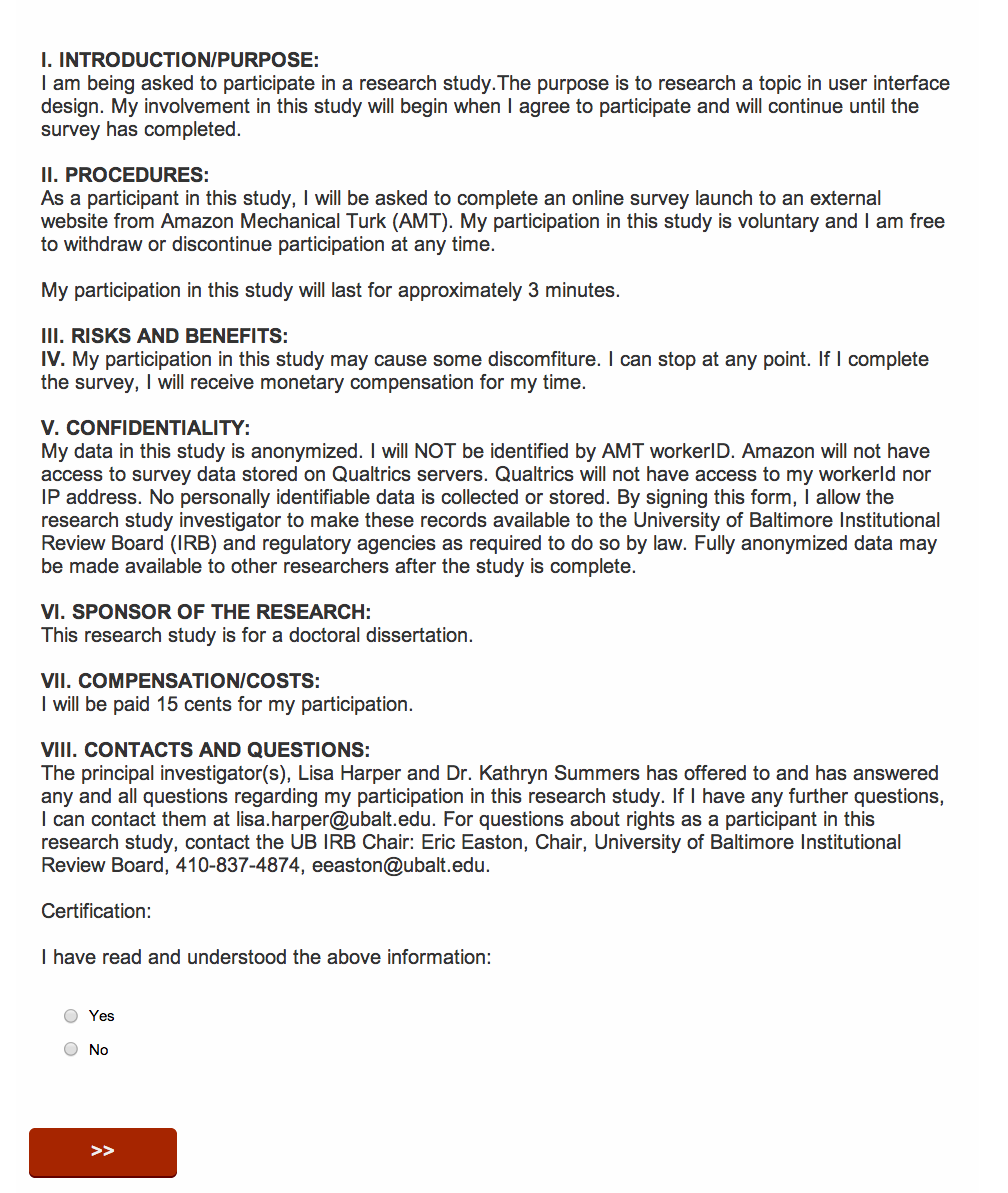
\includegraphics[scale=.40]{chapter4.tex/consent}
}
\end{figure}
%\setcounter{figure}{0} 
%
\chapter{AMT Terms of Service}
\label{amazon}
\begin{figure}[h!]
\centerline{
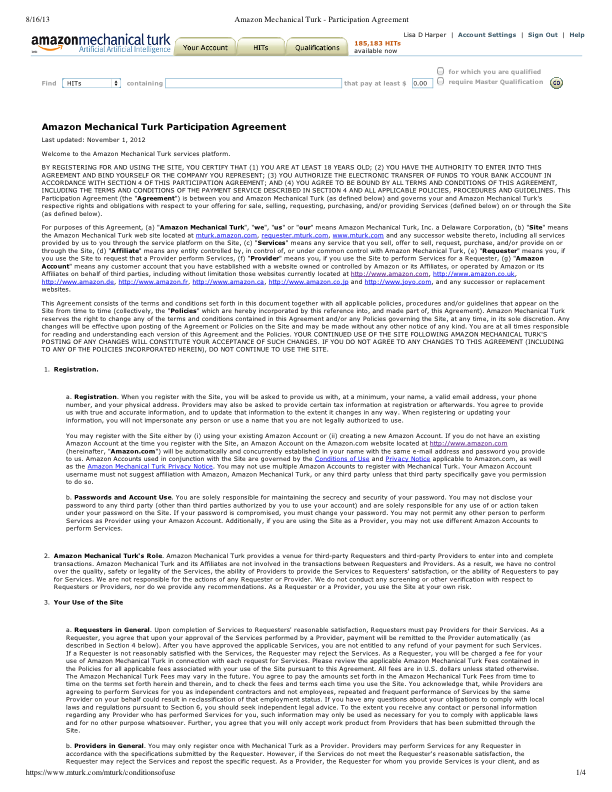
\includegraphics[scale=.6]{Appendices/amt-tos}
}
\end{figure}


%\setcounter{figure}{0} 
%
\chapter{Sample AMT Assignment Definition}
\label{assignment}
\lstset{numbers=none}
\begin{lstlisting}
title = Language study and demographic survey (3 min)
description: one task and then just a survey
keywords:survey, language

# how much you'll pay each subject
reward:.15

# how many subjects do you want
assignments:30

######################################
## HIT Timing Properties
######################################

# 60*10, 10 mins to finish a suvey
assignmentduration:600

# 60*60*24*2, 2 day to keep on mturk
hitlifetime:172800

# 10 seconds to auto approve the response
# 
autoapprovaldelay:10

######################################
## Qualification Properties
######################################

# user must have an approval rate of 90% or greater
qualification.1:000000000000000000L0
qualification.comparator.1:greaterthan
qualification.value.1:90
qualification.private.1:false

# user must be in the United States
qualification.2:00000000000000000071
qualification.comparator.2:equalto
qualification.locale.2:US
qualification.private.2:true
\end{lstlisting}


%\setcounter{figure}{0} 
%%**************************************************************
% Appendix
%*******************************************************
% If problems with the headers: get headings in appendix etc. right
%\markboth{\spacedlowsmallcaps{Appendix}}{\spacedlowsmallcaps{Appendix}}
\chapter{Survey Response}
\label{survey-response}
%%% LyX 2.0.6 created this file.  For more info, see http://www.lyx.org/.
%% Do not edit unless you really know what you are doing.
%\documentclass[english]{article}
%\usepackage[T1]{fontenc}
%\usepackage[latin9]{inputenc}
%\usepackage{longtable}
%\makeatletter

%%%%%%%%%%%%%%%%%%%%%%%%%%%%%% LyX specific LaTeX commands.
%% Because html converters don't know tabularnewline
%\providecommand{\tabularnewline}{\\}

%\makeatother

%\usepackage{babel}
%\begin{document}

%\setlength\LTleft{-30pt}            % default: \fill
%\setlength\LTright{-30pt}           % default: \fill
\footnotesize
\begin{longtable}{p{4cm} p{4cm}}
%\caption{Demographics (All Studies Combined)} \\
\textbf{Category} & \textbf{Percentage}\tabularnewline
\hline 
\hline 
\textbf{Age} & \tabularnewline
\hline 
18-24 & 28\%\tabularnewline
25-34 & 45\%\tabularnewline
35-49 & 20\%\tabularnewline
50-64 & 7\%\tabularnewline
64+ & 0\%\tabularnewline
\hline 
\textbf{Gender} & \tabularnewline
\hline 
Male & 53\%\tabularnewline
Female & 47\%\tabularnewline
\hline 
\textbf{Ethnic Identity} & \tabularnewline
\hline 
American Indian / Native American & 1\%\tabularnewline
Asian or Pacific Islander & 10\%\tabularnewline
Black / African American & 7\%\tabularnewline
Hispanic or Latin American & 7\%\tabularnewline
White / Caucasian & 73\%\tabularnewline
Near Eastern or Arabic & 0\%\tabularnewline
Other & 2\%\tabularnewline
\hline 
\textbf{Native Language} & \tabularnewline
\hline 
English & 97\%\tabularnewline
Other & 3\%\tabularnewline
\hline 
\textbf{English} & \tabularnewline
\hline 
A little English & 0\%\tabularnewline
Some English & 0\%\tabularnewline
Fluent English & 60\%\tabularnewline
Near-native English & 40\%\tabularnewline
\hline 
\textbf{Education} & \tabularnewline
\hline 
Some High School & 1\%\tabularnewline
High School Graduate & 13\%\tabularnewline
Some College / Associate Degree & 40\%\tabularnewline
College Degree & 37\%\tabularnewline
Post-graduate Degree & 9\%\tabularnewline
\hline 
\textbf{Income} & \tabularnewline
\hline 
Under 20,000 & 34\%\tabularnewline
20,000 - 30,000 & 19\%\tabularnewline
30,000 - 40,000 & 15\%\tabularnewline
40,000 - 50,000 & 10\%\tabularnewline
50,000+ & 22\%\tabularnewline
\hline 
\textbf{IT Job} & \tabularnewline
\hline
Yes & 20\%\tabularnewline
No & 80\%\tabularnewline
\hline 
\textbf{Internet Usage} & \tabularnewline
\hline 
Fewer than 4 hours per week & 2\%\tabularnewline
4-10 hours per week & 11\%\tabularnewline
10-25 hours per week & 30\%\tabularnewline
25+ hours per week & 57\%\tabularnewline
\hline 
\textbf{Shop Online} & \tabularnewline
\hline 
Never & 1\%\tabularnewline
Rarely & 17\%\tabularnewline
Sometimes & 30\%\tabularnewline
Often & 52\%\tabularnewline
\hline 
\textbf{Sense of Privacy in Public} & \tabularnewline
\hline 
Not private & 29\%\tabularnewline
A Little private & 30\%\tabularnewline
Somewhat private & 29\%\tabularnewline
Private & 9\%\tabularnewline
Very private & 3\%\tabularnewline
\hline 
\textbf{Sense of Privacy at Home} & \tabularnewline
\hline 
Not private & 4\%\tabularnewline
A Little private & 10\%\tabularnewline
Somewhat private & 23\%\tabularnewline
Private & 37\%\tabularnewline
Very private & 26\%\tabularnewline
\hline 
\textbf{Importance of Online Privacy } & \tabularnewline
\hline 
Not much of an issue & 7\%\tabularnewline
Somewhat important & 51\%\tabularnewline
Really important & 42\%\tabularnewline
\hline 
\textbf{Steps to Protect Privacy} & \tabularnewline
\hline 
Don't know how to protect & 8\%\tabularnewline
Know how but not consistent & 49\%\tabularnewline
Know how and take measures & 43\%\tabularnewline
\hline 
\textbf{Know what a tracking cookie is} & \tabularnewline
\hline 
Yes & 91\%\tabularnewline
No & 9\%\tabularnewline
\hline 
\textbf{DNT means...} & \tabularnewline
\hline 
Do not show targeted advertising & 20\%\tabularnewline
Do not track across sites & 54\%\tabularnewline
Do not track on this site & 47\%\tabularnewline
Do not collect information & 48\%\tabularnewline
Do not store information & 43\%\tabularnewline
\hline 
\textbf{Would Turn off Tracking if Easy?} & \tabularnewline
\hline 
Yes & 91\%\tabularnewline
No & 9\%\tabularnewline
\hline 
\textbf{Browser Configured Opt-Out} & \tabularnewline
\hline 
Yes & 55\%\tabularnewline
No & 45\%\tabularnewline
\hline 
\textbf{Use a Browser Plugin for Privacy Protection} & \tabularnewline
\hline 
Yes & 73\%\tabularnewline
No & 27\%\tabularnewline
\hline 
\textbf{Total} & \textbf{1158}\tabularnewline
\hline 
\end{longtable}
%\end{document}

%% LyX 2.0.6 created this file.  For more info, see http://www.lyx.org/.
%% Do not edit unless you really know what you are doing.
%\documentclass[english]{article}
%\usepackage[T1]{fontenc}
%\usepackage[latin9]{inputenc}

%\makeatletter

%%%%%%%%%%%%%%%%%%%%%%%%%%%%%% LyX specific LaTeX commands.
%% Because html converters don't know tabularnewline
%\providecommand{\tabularnewline}{\\}

%\makeatother

%\usepackage{babel}
%\begin{document}

\begin{longtable}{p{4cm} p{4cm} p{3cm}}
\caption{Aggregate Demographic Profile and Survey Response} \\
\textbf{Category} & \textbf{Experiment 3} & \textbf{Total}\tabularnewline
\hline 
\hline 
\textbf{Age} &  & \tabularnewline
\hline 
18-24 & 29\% & 28\%\tabularnewline
25-34 & 44\% & 45\%\tabularnewline
35-49 & 17\% & 20\%\tabularnewline
50-64 & 10\% & 7\%\tabularnewline
64+ & 0\% & 0\%\tabularnewline
\hline 
\textbf{Gender} &  & \tabularnewline
\hline 
Male & 63\% & 53\%\tabularnewline
Female & 37\% & 47\%\tabularnewline
\hline 
\textbf{Ethnic Identity} &  & \tabularnewline
\hline 
American Indian / Native American & 0\% & 1\%\tabularnewline
Asian or Pacific Islander & 10\% & 10\%\tabularnewline
Black / African American & 3\% & 7\%\tabularnewline
Hispanic or Latin American & 5\% & 7\%\tabularnewline
White / Caucasian & 82\% & 73\%\tabularnewline
Near Eastern or Arabic & 0\% & 0\%\tabularnewline
Other & 2\% & 2\%\tabularnewline
\hline 
\textbf{Native Language} &  & \tabularnewline
\hline 
English & 99\% & 97\%\tabularnewline
Other & 1\% & 3\%\tabularnewline
\hline 
\textbf{English} &  & \tabularnewline
\hline 
A little English & 0\% & 0\%\tabularnewline
Some English & 0\% & 0\%\tabularnewline
Fluent English & 0\% & 60\%\tabularnewline
Near-native English & 100\% & 40\%\tabularnewline
\hline 
\textbf{Education} &  & \tabularnewline
\hline 
Some High School & 1\% & 1\%\tabularnewline
High School Graduate & 17\% & 13\%\tabularnewline
Some College or Associate Degree & 39\% & 40\%\tabularnewline
College Degree & 35\% & 37\%\tabularnewline
Post-graduate Degree & 8\% & 9\%\tabularnewline
\hline 
\textbf{Income} &  & \tabularnewline
\hline 
Under 20,000 & 30\% & 34\%\tabularnewline
20,000 - 30,000 & 25\% & 19\%\tabularnewline
30,000 - 40,000 & 13\% & 15\%\tabularnewline
40,000 - 50,000 & 13\% & 10\%\tabularnewline
50,000+ & 20\% & 22\%\tabularnewline
\hline 
\textbf{IT Job} &  & \tabularnewline
\hline
Yes & 21\% & 20\%\tabularnewline
No & 79\% & 80\%\tabularnewline
\hline 
\textbf{Internet Usage} &  & \tabularnewline
\hline 
Fewer than 4 hours per week & 1\% & 2\%\tabularnewline
4-10 hours per week & 13\% & 11\%\tabularnewline
10-25 hours per week & 41\% & 30\%\tabularnewline
25+ hours per week & 45\% & 57\%\tabularnewline
\hline 
\textbf{Shop Online} &  & \tabularnewline
\hline 
Never & 1\% & 1\%\tabularnewline
Rarely & 20\% & 17\%\tabularnewline
Sometimes & 59\% & 30\%\tabularnewline
Often & 21\% & 52\%\tabularnewline
\hline 
\textbf{Sense of Privacy in Public} &  & \tabularnewline
\hline 
Not private & 31\% & 29\%\tabularnewline
A Little private & 34\% & 30\%\tabularnewline
Somewhat private & 23\% & 29\%\tabularnewline
Private & 11\% & 9\%\tabularnewline
Very prvate & 1\% & 3\%\tabularnewline
\hline 
\textbf{Sense of Privacy at Home} &  & \tabularnewline
\hline 
Not private & 5\% & 4\%\tabularnewline
A Little private & 15\% & 10\%\tabularnewline
Somewhat private & 23\% & 23\%\tabularnewline
Private & 34\% & 37\%\tabularnewline
Very prvate & 24\% & 26\%\tabularnewline
\hline 
\textbf{Importance of Online Privacy } &  & \tabularnewline
\hline 
Not much of an issue & 8\% & 7\%\tabularnewline
Somewhat important & 50\% & 51\%\tabularnewline
Really important & 42\% & 42\%\tabularnewline
\hline 
\textbf{Steps to Protect Privacy} &  & \tabularnewline
\hline 
Don't know how to protect & 12\% & 8\%\tabularnewline
Know how but not consistent & 38\% & 49\%\tabularnewline
Know how and take measures & 50\% & 43\%\tabularnewline
\hline 
\textbf{Know what a tracking cookie is} &  & \tabularnewline
\hline 
Yes & 90\% & 91\%\tabularnewline
No & 10\% & 9\%\tabularnewline
\hline 
\textbf{DNT means...} &  & \tabularnewline
\hline 
Do not show targeted advertising & 17\% & 20\%\tabularnewline
Do not trakc across sites & 44\% & 54\%\tabularnewline
Do not track on this site & 49\% & 47\%\tabularnewline
Do not collect information & 39\% & 48\%\tabularnewline
Do not store information & 38\% & 43\%\tabularnewline
\hline 
\textbf{Would Turn off Tracking if Easy?} &  & \tabularnewline
\hline 
Yes & 88\% & 91\%\tabularnewline
No & 12\% & 9\%\tabularnewline
\hline 
\textbf{Browser Configured Opt-Out} &  & \tabularnewline
\hline 
Yes & 54\% & 55\%\tabularnewline
No & 46\% & 45\%\tabularnewline
\hline 
\textbf{Use a Browser Plugin for Privacy Protection} &  & \tabularnewline
\hline 
Yes & 70\% & 73\%\tabularnewline
No & 30\% & 27\%\tabularnewline
\hline 
\textbf{Total} & \textbf{100} & \textbf{1158}\tabularnewline
\end{longtable}
%\end{document}

%\setcounter{figure}{0} 
%
\chapter{Experiment 1 Conditions}
\label{exp1-conditions}
\begin{figure}[h!]
\centerline{
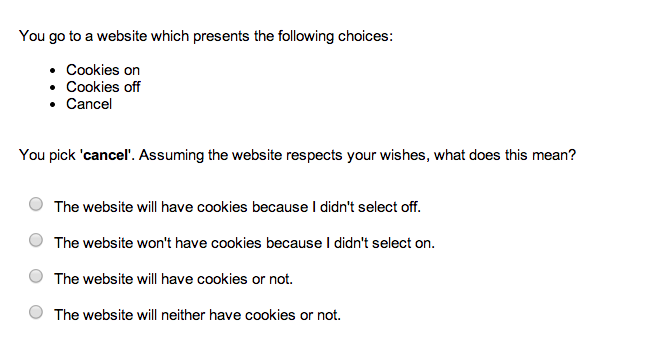
\includegraphics[scale=.5]{chapter5.tex/textnocpcookie}
}
\caption{Text, No Deontic Force, Cookie Condition}
\end{figure}


\begin{figure}[h!]
\centerline{
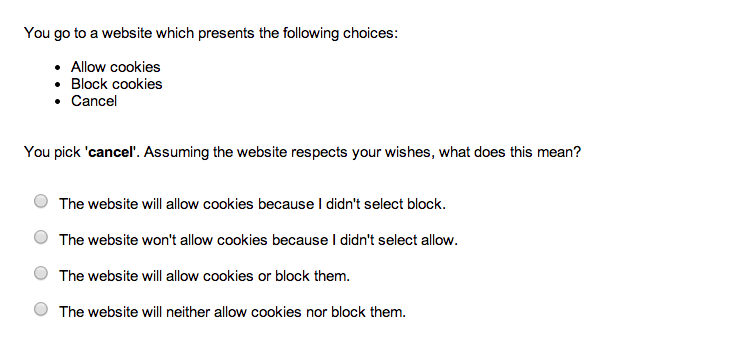
\includegraphics[scale=.5]{chapter5.tex/textcpcookie}
}
\caption{Text, Deontic Force, Cookie Condition}
\end{figure}


\begin{figure}[h!]
\centerline{
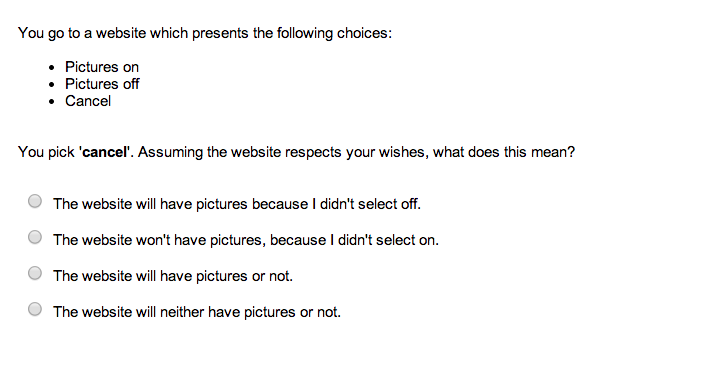
\includegraphics[scale=.5]{chapter5.tex/textnocppic}
}
\caption{Text, No Deontic Force, Picture Condition}
\end{figure}


\begin{figure}[h!]
\centerline{
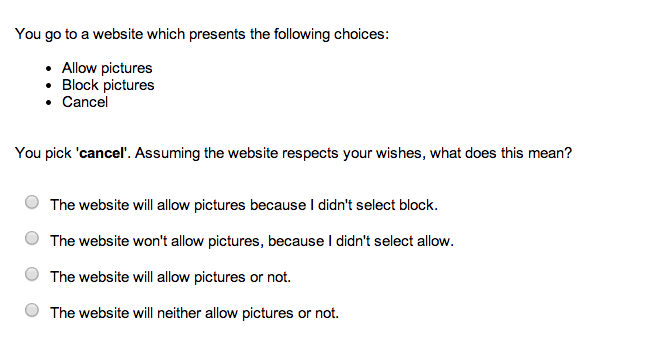
\includegraphics[scale=.5]{chapter5.tex/textcppic}
}
\caption{Text, Deontic Force, Picture Condition}
\end{figure}


\begin{figure}[h!]
\centerline{
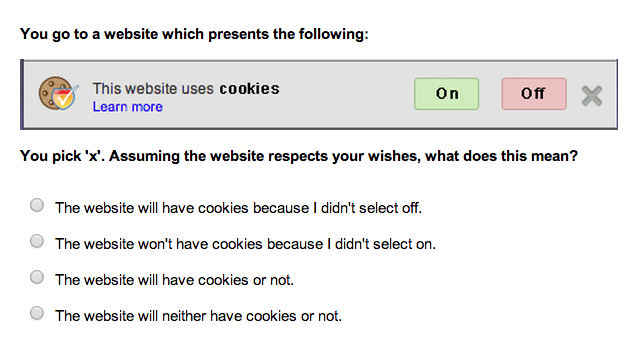
\includegraphics[scale=.5]{chapter5.tex/dialognocpcookie}
}
\caption{Mixed-Modal, No Deontic Force, Cookie Condition}
\end{figure}


\begin{figure}[h!]
\centerline{
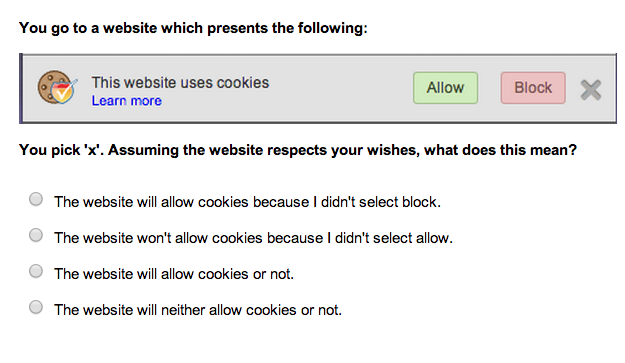
\includegraphics[scale=.5]{chapter5.tex/dialogcpcookie}
}
\caption{Mixed-Modal, Deontic Force, Cookie Condition}
\end{figure}



\begin{figure}[h!]
\centerline{
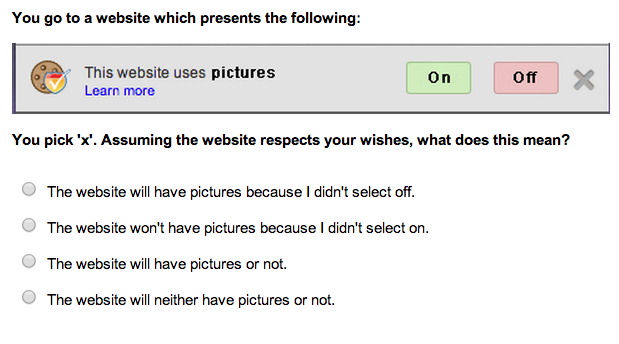
\includegraphics[scale=.5]{chapter5.tex/dialognocppic}
}
\caption{Mixed-Modal, No Deontic Force, Picture Condition}
\end{figure}


\begin{figure}[h!]
\centerline{
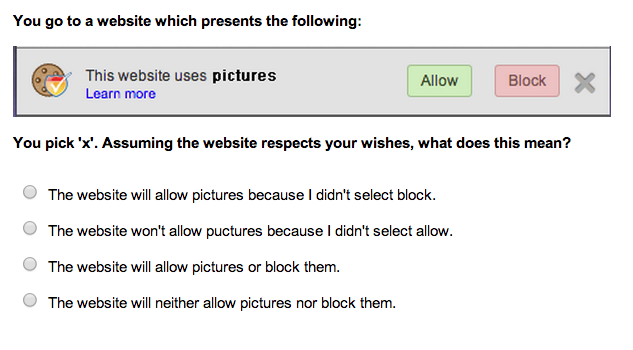
\includegraphics[scale=.5]{chapter5.tex/dialogcppic}
}
\caption{Mixed-Modal, Deontic Force, Picture Condition}
\end{figure}
%\setcounter{figure}{0} 
%
\chapter{Experiment 1 Raw Results}
\label{exp1-raw}
\begin{figure}[h!]
\centerline{
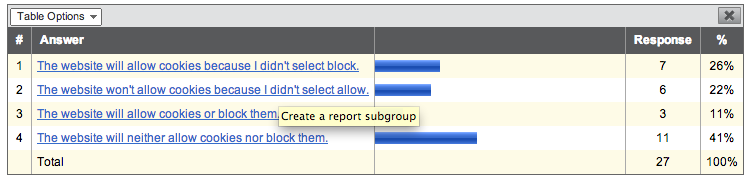
\includegraphics[scale=.44]{chapter5.tex/raw1}
}
\caption{Text, Deontic Force, Cookie Condition}
\end{figure}


\begin{figure}[h!]
\centerline{
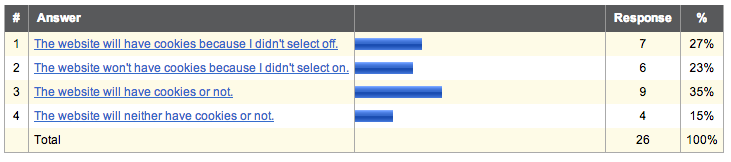
\includegraphics[scale=.45]{chapter5.tex/raw2}
}
\caption{Text, No Deontic Force, Cookie Condition}
\end{figure}


\begin{figure}[h!]
\centerline{
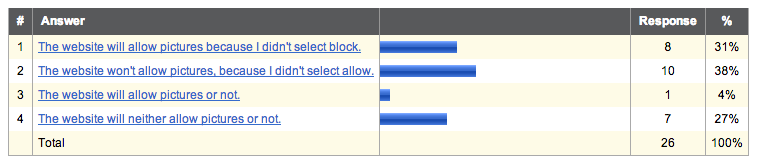
\includegraphics[scale=.45]{chapter5.tex/raw3}
}
\caption{Text, Deontic Force, Picture Condition}
\end{figure}


\begin{figure}[h!]
\centerline{
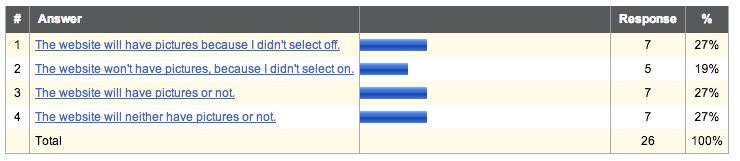
\includegraphics[scale=.45]{chapter5.tex/raw4}
}
\caption{Text, No Deontic Force, Picture Condition}
\end{figure}


\begin{figure}[h!]
\centerline{
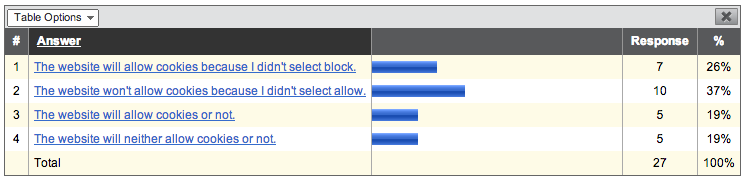
\includegraphics[scale=.44]{chapter5.tex/raw5}
}
\caption{Graphic, Deontic Force, Cookie Condition}
\end{figure}


\begin{figure}[h!]
\centerline{
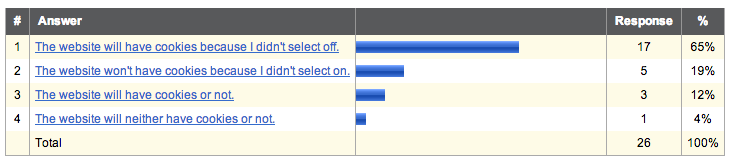
\includegraphics[scale=.45]{chapter5.tex/raw6}
}
\caption{Graphic, No Deontic Force, Cookie Condition}
\end{figure}


\begin{figure}[h!]
\centerline{
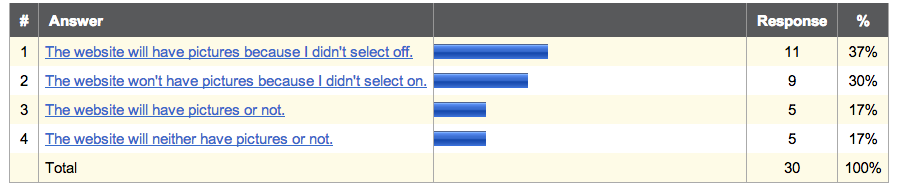
\includegraphics[scale=.38]{chapter5.tex/raw7}
}
\caption{Graphic, No Deontic Force, Picture Condition}
\end{figure}


\begin{figure}[h!]
\centerline{
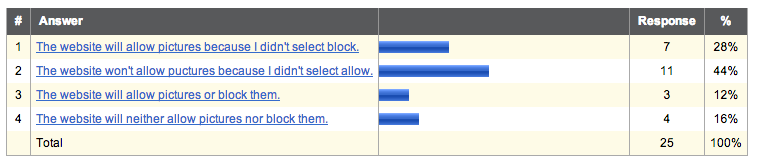
\includegraphics[scale=.45]{chapter5.tex/raw8}
}
\caption{Graphic, Deontic Force, Picture Condition}
\end{figure}
%\setcounter{figure}{0} 
%
\chapter{Participant Survey}
\label{survey}
%\begin{parbox}{\textwidth}
%\centering
%\begin{figure}
%\begin{sideways}
%\centerline{
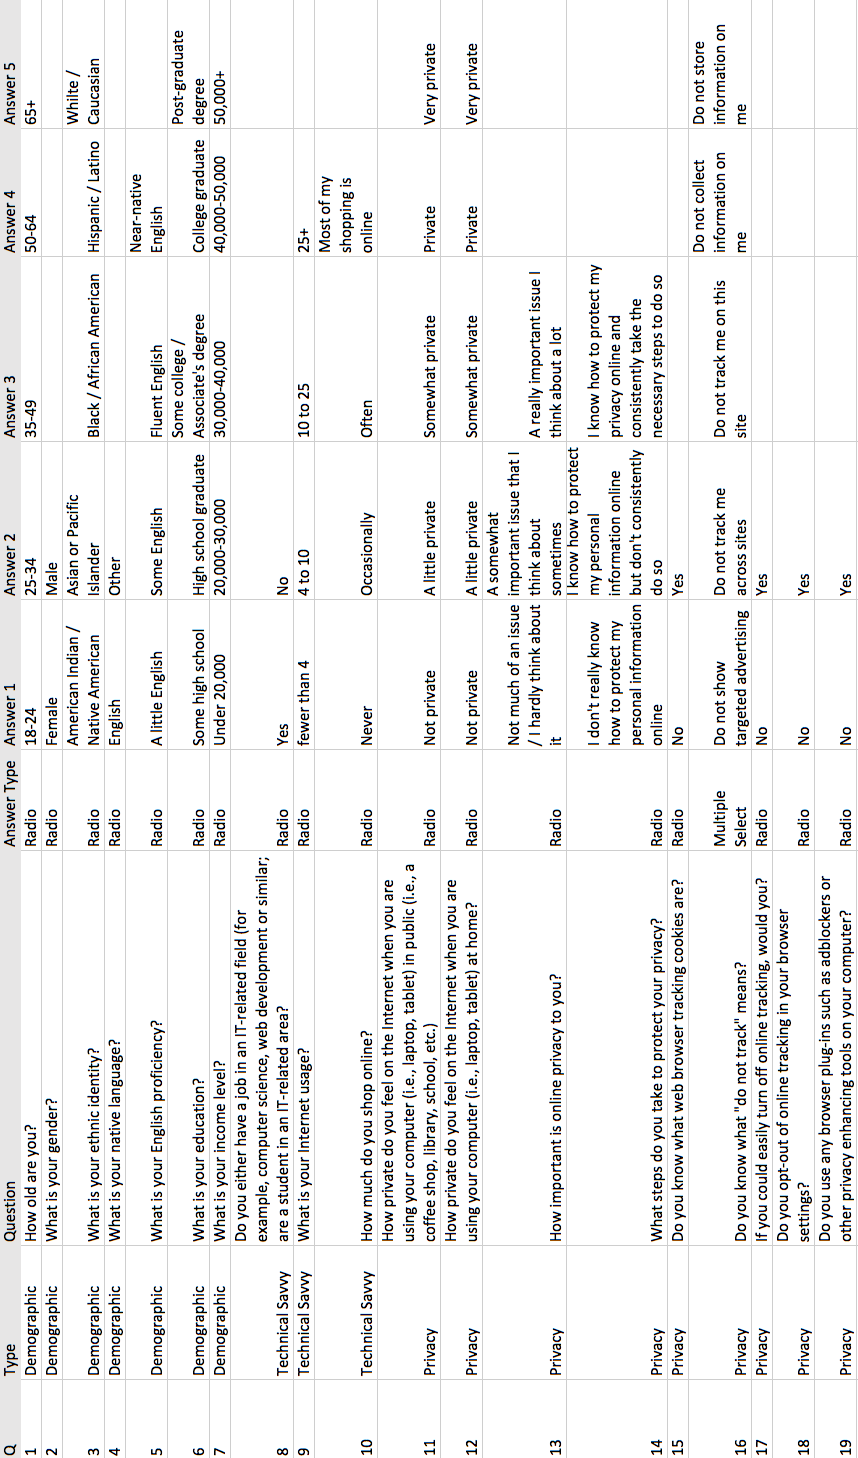
\includegraphics[scale=.38]{Appendices/survey-rotated}
%}
%\end{sideways}
%\end{figure}
%\end{parbox}

 %

%----------------------------------------------------------------------------------------
%	POST-CONTENT THESIS PAGES
%----------------------------------------------------------------------------------------

\cleardoublepage% Bibliography

\label{app:bibliography} % Reference the bibliography elsewhere with \autoref{app:bibliography}

\manualmark
\markboth{\spacedlowsmallcaps{\bibname}}{\spacedlowsmallcaps{\bibname}} 
\refstepcounter{dummy}

\addtocontents{toc}{\protect\vspace{\beforebibskip}} % Place the bibliography slightly below the rest of the document content in the table of contents
\addcontentsline{toc}{chapter}{\tocEntry{\bibname}}

%\bibliographystyle{plainnat}
%\bibliographystyle{apalike2}
\bibliographystyle{apacite}

%\bibliography{Bibliography}
\bibliography{bib} % Bibliography

\end{document}